\section{Iterations} 

\subsection{\colorbox{violet}{Project Sprints}}

\begin{table}[!hbt]
\begin{tabular}{|c|c|c|c|}
\hline
\textbf{Sprint \#} & \textbf{Remainder (pts)} & \textbf{Planned (pts)} & \textbf{\begin{tabular}[c]{@{}c@{}}Completed (pts)\\ (Speed)\end{tabular}} \\ \hline
Sprint 1 & 39 & 12 & 8  \\ \hline
Sprint 2 & 31 & 21 & 21 \\ \hline
Sprint 3 & 10 & 10 & 10 \\ \hline
\end{tabular}
\end{table}
\label{sprints}

\subsection{Sprint 1}

\subsubsection{Plan}
In this sprint we aimed to get a simple working version of Blackjack that runs from a GUI.

\noindent We added 6 (Main, card, deck, hand, player, and game).java that serves as our business logic for our game. Additionally we added a login screen that allows the user to sign in, create an account, or play as a guest. We have also implemented the base for our backend database that stores our users login info.

\subsubsection{Activities (Stories)}

\textbf{Beginning of Sprint 1 (Paired Programming)}

\begin{table}[!hbt]
\begin{tabular}{|l|l|}
\hline
\multicolumn{1}{|c|}{\textbf{Name (pts)}} & \multicolumn{1}{c|}{\textbf{Stories Attempted (pts)}} \\ \hline
Chris, Callie (5)                         & S14(1), S21(1), S26(3)                                \\ \hline
Jenna, Emma (7)                           & S1(2), S2(1), S3(2), S7(2)                            \\ \hline
\end{tabular}
\end{table}
\label{sprint 1 planned stories}



\noindent \textbf{End of Sprint 1 (Paired Programming)}

\begin{table}[!hbt]
\begin{tabular}{|l|l|}
\hline
\multicolumn{1}{|c|}{\textbf{Name (pts)}} & \multicolumn{1}{c|}{\textbf{Stories Accomplished (pts)}} \\ \hline
Chris, Callie (4) & S21(1),  S26(3) \\ \hline
Jenna, Emma (4) & S1(2), S3(2) \\ \hline
\end{tabular}
\end{table}
\label{end of sprint 1}

\pagebreak

\noindent \textbf{Individual Speeds and Cycle times}

\begin{table}[!hbt]
\begin{tabular}{|c|c|c|c|c|}
\hline
\textbf{Name} &
  \textbf{\begin{tabular}[c]{@{}c@{}}Speed\\ (pts)\end{tabular}} &
  \textbf{\begin{tabular}[c]{@{}c@{}}Paired \\ Programming\\ ($\div 2$)\end{tabular}} &
  \textbf{\begin{tabular}[c]{@{}c@{}}Work \\ (hrs)\end{tabular}} &
  \textbf{\begin{tabular}[c]{@{}c@{}}Cycle\\ (hrs/pts)\end{tabular}} \\ \hline
Chris  & 4 & 2 & 35 & 16   \\ \hline
Jenna  & 4 & 2 & 40 & 20   \\ \hline
Callie & 4 & 2 & 35 & 17.5 \\ \hline
Emma   & 4 & 2 & 29 & 14.5 \\ \hline
\end{tabular}
\end{table}
\label{sprint 1 speed}

\subsubsection{Sprint 1 Testing}

Here are the individual testing results for each member:

\begin{table}[!hbt]
\begin{tabular}{|ccc|}
\hline
\multicolumn{1}{|c|}{\textbf{Class}}                                              & \multicolumn{1}{c|}{\textbf{Statement Coverage (\%)}} & \textbf{Branch Coverage (\%)} \\ \hline
\multicolumn{3}{|c|}{\textbf{Chris}}                                                                                                 \\ \hline
\multicolumn{1}{|c|}{Card}                                                      & \multicolumn{1}{c|}{100}           & 100           \\ \hline
\multicolumn{1}{|c|}{Deck}                                                      & \multicolumn{1}{c|}{100}           & 100           \\ \hline
\multicolumn{1}{|c|}{Game}                                                      & \multicolumn{1}{c|}{80}            & 70            \\ \hline
\multicolumn{1}{|c|}{Hand}                                                      & \multicolumn{1}{c|}{97}            & 93            \\ \hline
\multicolumn{1}{|c|}{Player}                                                    & \multicolumn{1}{c|}{100}           & 100           \\ \hline
\multicolumn{1}{|c|}{\textbf{Average}}                                          & \multicolumn{1}{c|}{\textbf{95.4}} & \textbf{92.6} \\ \hline
\multicolumn{3}{|c|}{\textbf{Jenna}}                                                                                                 \\ \hline
\multicolumn{1}{|c|}{\begin{tabular}[c]{@{}c@{}}User\\ Controller\end{tabular}} & \multicolumn{1}{c|}{74}            & 62            \\ \hline
\multicolumn{1}{|c|}{\begin{tabular}[c]{@{}c@{}}Logout\\ Controller\end{tabular}} & \multicolumn{1}{c|}{100}                              & 100                           \\ \hline
\multicolumn{1}{|c|}{\textbf{Average}}                                          & \multicolumn{1}{c|}{\textbf{87}}   & \textbf{81}   \\ \hline
\multicolumn{3}{|c|}{\textbf{Callie}}                                                                                                \\ \hline
\multicolumn{1}{|c|}{\begin{tabular}[c]{@{}c@{}}Game\\ Controller\end{tabular}} & \multicolumn{1}{c|}{91}            & 77            \\ \hline
\multicolumn{1}{|c|}{\textbf{Average}}                                          & \multicolumn{1}{c|}{\textbf{91}}   & \textbf{77}   \\ \hline
\multicolumn{3}{|c|}{\textbf{Emma}}                                                                                                  \\ \hline
\multicolumn{1}{|c|}{App/page}                                                  & \multicolumn{1}{c|}{100}           & 100           \\ \hline
\multicolumn{1}{|c|}{\textbf{Average}}                                          & \multicolumn{1}{c|}{\textbf{100}}  & \textbf{100}  \\ \hline
\end{tabular}
\end{table}
\label{sprint 1 testing}

\pagebreak

\subsubsection{(Sprint 1) Retrospective}
We realized that integration between model, view and controller can take much more time than anticipated. Additionally, some of our original point values for our user stories might have been underestimated.

\subsection{\colorbox{cyan}{Sprint 2}}


\subsubsection{\colorbox{cyan}{Plan}}

\noindent Our plan for sprint 2 was to develop the social aspects of the game around our simple functioning version of our game. This included more robust sign in/out, guest user handling, messaging and friend management. We implemented numerous java script and css files that build our GUI using data in our database.

\subsubsection{\colorbox{cyan}{Activities (Stories)}}

\textbf{Beginning of Sprint 2}

\begin{table}[!hbt]
\begin{tabular}{|l|l|}
\hline
\multicolumn{1}{|c|}{\textbf{Name (pts)}} & \multicolumn{1}{c|}{\textbf{Stories Attempted (pts)}} \\ \hline
Chris (7)  & S8(2), S10(2), S12(2), T3(1)       \\ \hline
Jenna (7)  & S2(1), S4(1), S5(1), S6(1), S7(2), T1(1) \\ \hline
Callie (6) & S15(1), S22(2), S23(2), T2(1)              \\ \hline
Emma (5)   & S19(2), S20(2), T4(1)               \\ \hline
\end{tabular}
\end{table}
\label{start sprint 2}

\noindent \textbf{End of Sprint 2}

\begin{table}[!hbt]
\begin{tabular}{|l|l|}
\hline
\multicolumn{1}{|c|}{\textbf{Name (pts)}} & \multicolumn{1}{c|}{\textbf{Stories Accomplished (pts)}} \\ \hline
Chris (9)  & S8(2), S9(2), S10(2), S11(2), T3(1) \\ \hline
Jenna (6)  & S2(1), S4(1), S5(1), S7(2), T1(1)   \\ \hline
Callie (5) & S22(2), S23(2), T2(1)             \\ \hline
Emma (5)   & S19(2), S20(2), T4(1)         \\ \hline
\end{tabular}
\end{table}
\label{end sprint 2}

\pagebreak

\noindent \textbf{Individual Speeds and Cycle times}

\begin{table}[!hbt]
\begin{tabular}{|c|c|c|c|}
\hline
\textbf{Name} &
  \textbf{\begin{tabular}[c]{@{}c@{}}Speed\\ (pts)\end{tabular}} &
  \textbf{\begin{tabular}[c]{@{}c@{}}Work \\ (hrs)\end{tabular}} &
  \textbf{\begin{tabular}[c]{@{}c@{}}Cycle\\ (hrs/pts)\end{tabular}} \\ \hline
Chris  & 9 & 35 & 3.89  \\ \hline
Jenna  & 6 & 30 & 5     \\ \hline
Callie & 5 & 45 & 9     \\ \hline
Emma   & 5 & 15 & 3     \\ \hline
\end{tabular}
\end{table}
\label{sprint 2 speed}

\subsubsection{\colorbox{cyan}{Sprint 2 Testing}}

Here are the individual testing results for each member:

\begin{table}[!hbt]
\begin{tabular}{|ccc|}
\hline
\multicolumn{1}{|c|}{\textbf{Class}} & \multicolumn{1}{c|}{\textbf{Statement Coverage (\%)}} & \textbf{Branch Coverage (\%)} \\ \hline
\multicolumn{3}{|c|}{\textbf{Chris}}                                                          \\ \hline
\multicolumn{1}{|c|}{TableList}          & \multicolumn{1}{c|}{100}           & 100           \\ \hline
\multicolumn{1}{|c|}{TableInfo}          & \multicolumn{1}{c|}{100}           & 100           \\ \hline
\multicolumn{1}{|c|}{JoinTable}          & \multicolumn{1}{c|}{96}            & 92            \\ \hline
\multicolumn{1}{|c|}{CreateTable}        & \multicolumn{1}{c|}{80}            & 62            \\ \hline
\multicolumn{1}{|c|}{{[}tableId{]}/page} & \multicolumn{1}{c|}{100}           & 100           \\ \hline
\multicolumn{1}{|c|}{\textbf{Average}}   & \multicolumn{1}{c|}{\textbf{95.2}} & \textbf{90.8} \\ \hline
\multicolumn{3}{|c|}{\textbf{Jenna}}                                                          \\ \hline
\multicolumn{1}{|c|}{ManageFriends}      & \multicolumn{1}{c|}{100}           & 100           \\ \hline
\multicolumn{1}{|c|}{FriendsList}        & \multicolumn{1}{c|}{85.4}          & 70            \\ \hline
\multicolumn{1}{|c|}{UserList}           & \multicolumn{1}{c|}{92.8}          & 75            \\ \hline
\multicolumn{1}{|c|}{\textbf{Average}}   & \multicolumn{1}{c|}{\textbf{92.7}} & \textbf{81.7} \\ \hline
\multicolumn{3}{|c|}{\textbf{Callie}}                                                         \\ \hline
\multicolumn{1}{|c|}{CardDisplay}        & \multicolumn{1}{c|}{65}            & 75.5          \\ \hline
\multicolumn{1}{|c|}{\textbf{Average}}   & \multicolumn{1}{c|}{\textbf{65}}   & \textbf{75.5} \\ \hline
\multicolumn{3}{|c|}{\textbf{Emma}}                                                           \\ \hline
\multicolumn{1}{|c|}{Context/auth}       & \multicolumn{1}{c|}{89.1}          & 80            \\ \hline
\multicolumn{1}{|c|}{Loading}            & \multicolumn{1}{c|}{100}           & 100           \\ \hline
\multicolumn{1}{|c|}{layout}             & \multicolumn{1}{c|}{88.6}          & 57.1          \\ \hline
\multicolumn{1}{|c|}{Stats}              & \multicolumn{1}{c|}{89.7}          & 80            \\ \hline
\multicolumn{1}{|c|}{Login}              & \multicolumn{1}{c|}{91.6}          & 71.4          \\ \hline
\multicolumn{1}{|c|}{SignUp}             & \multicolumn{1}{c|}{93.2}          & 90            \\ \hline
\multicolumn{1}{|c|}{\textbf{Average}}   & \multicolumn{1}{c|}{\textbf{92}}   & \textbf{79.8} \\ \hline
\end{tabular}
\end{table}
\label{sprint 2 testing}


\begin{figure}[!hbt]
    \centering
    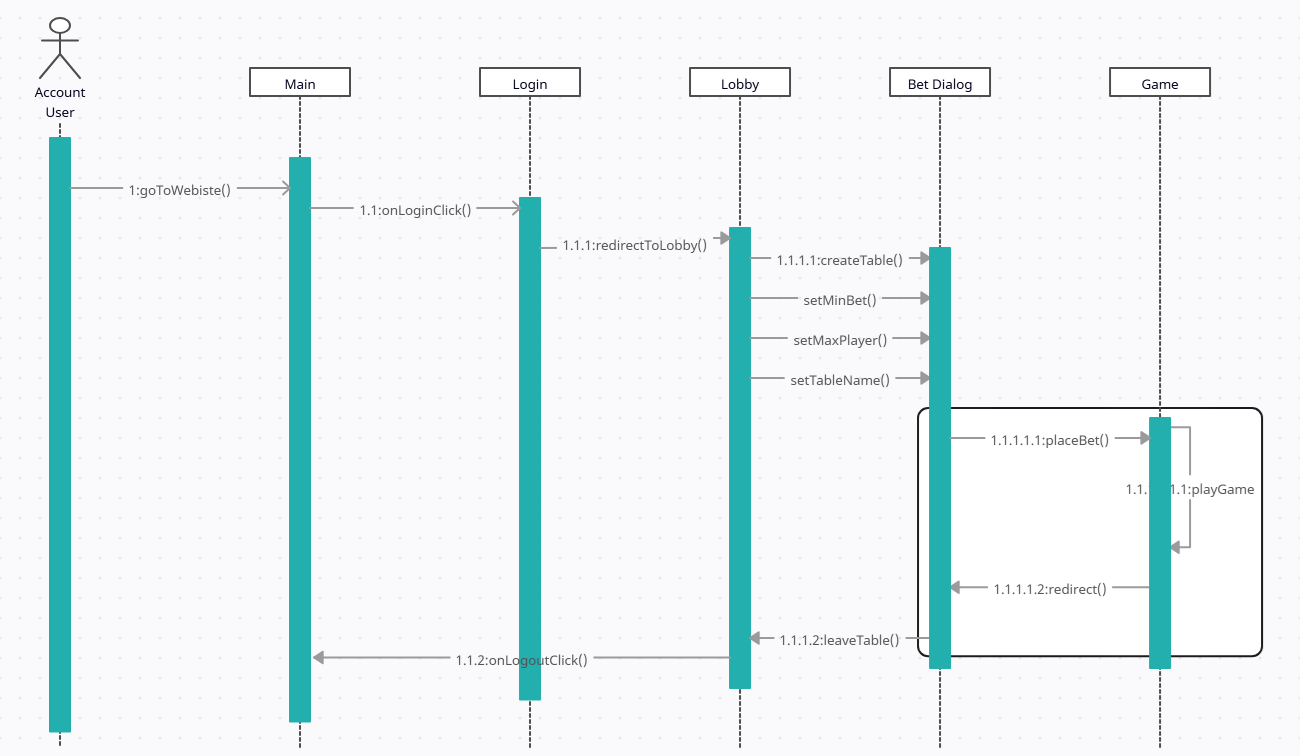
\includegraphics[width=1.0\linewidth]{figures/sequence.png}
    \caption{Sequence Diagram for a user playing the game}
    \label{fig:sequence}
\end{figure}

\ref{fig:sequence}This is the sequence diagram for a user signing in and playing a game of blackjack. 

\subsubsection{\colorbox{cyan}{(Sprint 2) Retrospective}}
In this sprint we realized multiple things including the importance of planning stories. We were fortunate that we planned our stories based on core components of the app. Sprint 1 was focused on the model components of the app allowing us to build all the of the social aspects of the app on top of the existing model components. Additionally, we realized the importance of having the "main" branch be the most current working version of our project. Each member should push to their branch and then move it to main so that everyone else pulls from main rather than pulling from each other. This ensures that main is always up to date and compiles. We also switched our database from MySQL to Firestore/Firebase. This was a good switch as we were having a lot of trouble with MySQL and Firebase was not only easy to use, but thanks to Jenna it was easy to covert to. 


\subsection{\colorbox{violet}{Sprint 3}}

\subsubsection{\colorbox{violet}{Plan}}

\noindent After our last sprint we only had a few stories left to do that centered on admin privileges, table messaging and full multiplayer functionality.

\subsubsection{\colorbox{violet}{Activities (Stories)}}

\textbf{Beginning of Sprint 3}

\begin{table}[!hbt]
\begin{tabular}{|l|l|}
\hline
\multicolumn{1}{|c|}{\textbf{Name (pts)}} & \multicolumn{1}{c|}{\textbf{Stories Attempted (pts)}} \\ \hline
Chris (3)  & S12 (2), T6 (1)        \\ \hline
Jenna (5)  & S6 (1), S24 (2) T5 (1) \\ \hline
Callie (3) & S15 (1), S17 (2)       \\ \hline
Emma (3)   & S25 (2), T5 (1)        \\ \hline
\end{tabular}
\end{table}
\label{start sprint 3}

\noindent \textbf{End of Sprint 3}

\begin{table}[!hbt]
\begin{tabular}{|l|l|}
\hline
\multicolumn{1}{|c|}{\textbf{Name (pts)}} & \multicolumn{1}{c|}{\textbf{Stories Attempted (pts)}} \\ \hline
Chris (3)  & S12 (2), T6 (1)        \\ \hline
Jenna (5)  & S6 (1), S24 (2) T5 (1) \\ \hline
Callie (3) & S15 (1), S17 (2)       \\ \hline
Emma (3)   & S25 (2), T5 (1)        \\ \hline
\end{tabular}
\end{table}
\label{end sprint 3}

\noindent \textbf{Individual Speeds and Cycle times}

\begin{table}[!hbt]
\begin{tabular}{|c|c|c|c|}
\hline
\textbf{Name} &
  \textbf{\begin{tabular}[c]{@{}c@{}}Speed\\ (pts)\end{tabular}} &
  \textbf{\begin{tabular}[c]{@{}c@{}}Work \\ (hrs)\end{tabular}} &
  \textbf{\begin{tabular}[c]{@{}c@{}}Cycle\\ (hrs/pts)\end{tabular}} \\ \hline
Chris  & 3 & 56 & 18.67 \\ \hline
Jenna  & 5 & 10 & 2     \\ \hline
Callie & 3 & 15  & 5     \\ \hline
Emma   & 3 & 11 & 3.67  \\ \hline
\end{tabular}
\end{table}
\label{end of sprint 3}

\pagebreak

\subsubsection{\colorbox{violet}{Sprint 3 Testing}}

Here are the individual testing results for each member: 

\begin{table}[!hbt]
\begin{tabular}{|ccc|}
\hline
\multicolumn{1}{|c|}{\textbf{Class}} & \multicolumn{1}{c|}{\textbf{Statement Coverage (\%)}} & \textbf{Branch Coverage (\%)} \\ \hline
\multicolumn{3}{|c|}{\textbf{Chris}}                                                          \\ \hline
\multicolumn{1}{|c|}{CardDisplay}      & \multicolumn{1}{c|}{64.25}          & 61.37          \\ \hline
\multicolumn{1}{|c|}{\textbf{Average}} & \multicolumn{1}{c|}{\textbf{64.25}} & \textbf{61.37} \\ \hline
\multicolumn{3}{|c|}{\textbf{Jenna}}                                                          \\ \hline
\multicolumn{1}{|c|}{ManageFriends}    & \multicolumn{1}{c|}{94.1}           & 84.21          \\ \hline
\multicolumn{1}{|c|}{FriendsList}      & \multicolumn{1}{c|}{100}            & 100            \\ \hline
\multicolumn{1}{|c|}{UserList}         & \multicolumn{1}{c|}{100}            & 100            \\ \hline
\multicolumn{1}{|c|}{Auth}             & \multicolumn{1}{c|}{100}            & 100            \\ \hline
\multicolumn{1}{|c|}{\textbf{Average}} & \multicolumn{1}{c|}{\textbf{98.52}} & \textbf{96.05} \\ \hline
\multicolumn{3}{|c|}{\textbf{Callie}}                                                         \\ \hline
\multicolumn{1}{|c|}{AuthContext}      & \multicolumn{1}{c|}{100}            & 100            \\ \hline
\multicolumn{1}{|c|}{ChatContext}      & \multicolumn{1}{c|}{91.66}          & 66.66          \\ \hline
\multicolumn{1}{|c|}{Chat}             & \multicolumn{1}{c|}{83.33}          & 66.66          \\ \hline
\multicolumn{1}{|c|}{ChatBox}          & \multicolumn{1}{c|}{100}            & 100            \\ \hline
\multicolumn{1}{|c|}{List}             & \multicolumn{1}{c|}{80}             & 100            \\ \hline
\multicolumn{1}{|c|}{ChatList}         & \multicolumn{1}{c|}{88.09}          & 55.55          \\ \hline
\multicolumn{1}{|c|}{AddUser}          & \multicolumn{1}{c|}{84.33}          & 69.23          \\ \hline
\multicolumn{1}{|c|}{UserInfo}         & \multicolumn{1}{c|}{100}            & 100            \\ \hline
\multicolumn{1}{|c|}{TableChat}        & \multicolumn{1}{c|}{88.67}          & 66.66          \\ \hline
\multicolumn{1}{|c|}{\textbf{Average}} & \multicolumn{1}{c|}{\textbf{91.89}} & \textbf{80.53} \\ \hline
\multicolumn{3}{|c|}{\textbf{Emma}}                                                           \\ \hline
\multicolumn{1}{|c|}{AllUsers}         & \multicolumn{1}{c|}{100}            & 100            \\ \hline
\multicolumn{1}{|c|}{SelectedUser}     & \multicolumn{1}{c|}{100}            & 92.85          \\ \hline
\multicolumn{1}{|c|}{ManageUsers}      & \multicolumn{1}{c|}{95.23}          & 80             \\ \hline
\multicolumn{1}{|c|}{\textbf{Average}} & \multicolumn{1}{c|}{\textbf{98.41}} & \textbf{90.95} \\ \hline
\end{tabular}
\end{table}
\label{sprint 3 testing}

\noindent Note that the CardDisplay component is the front end for our app which has a lot of response checking from the backend that couldnt be covered from an invalid response perspective thus the low coverage.

\pagebreak


\begin{figure}
    \centering
    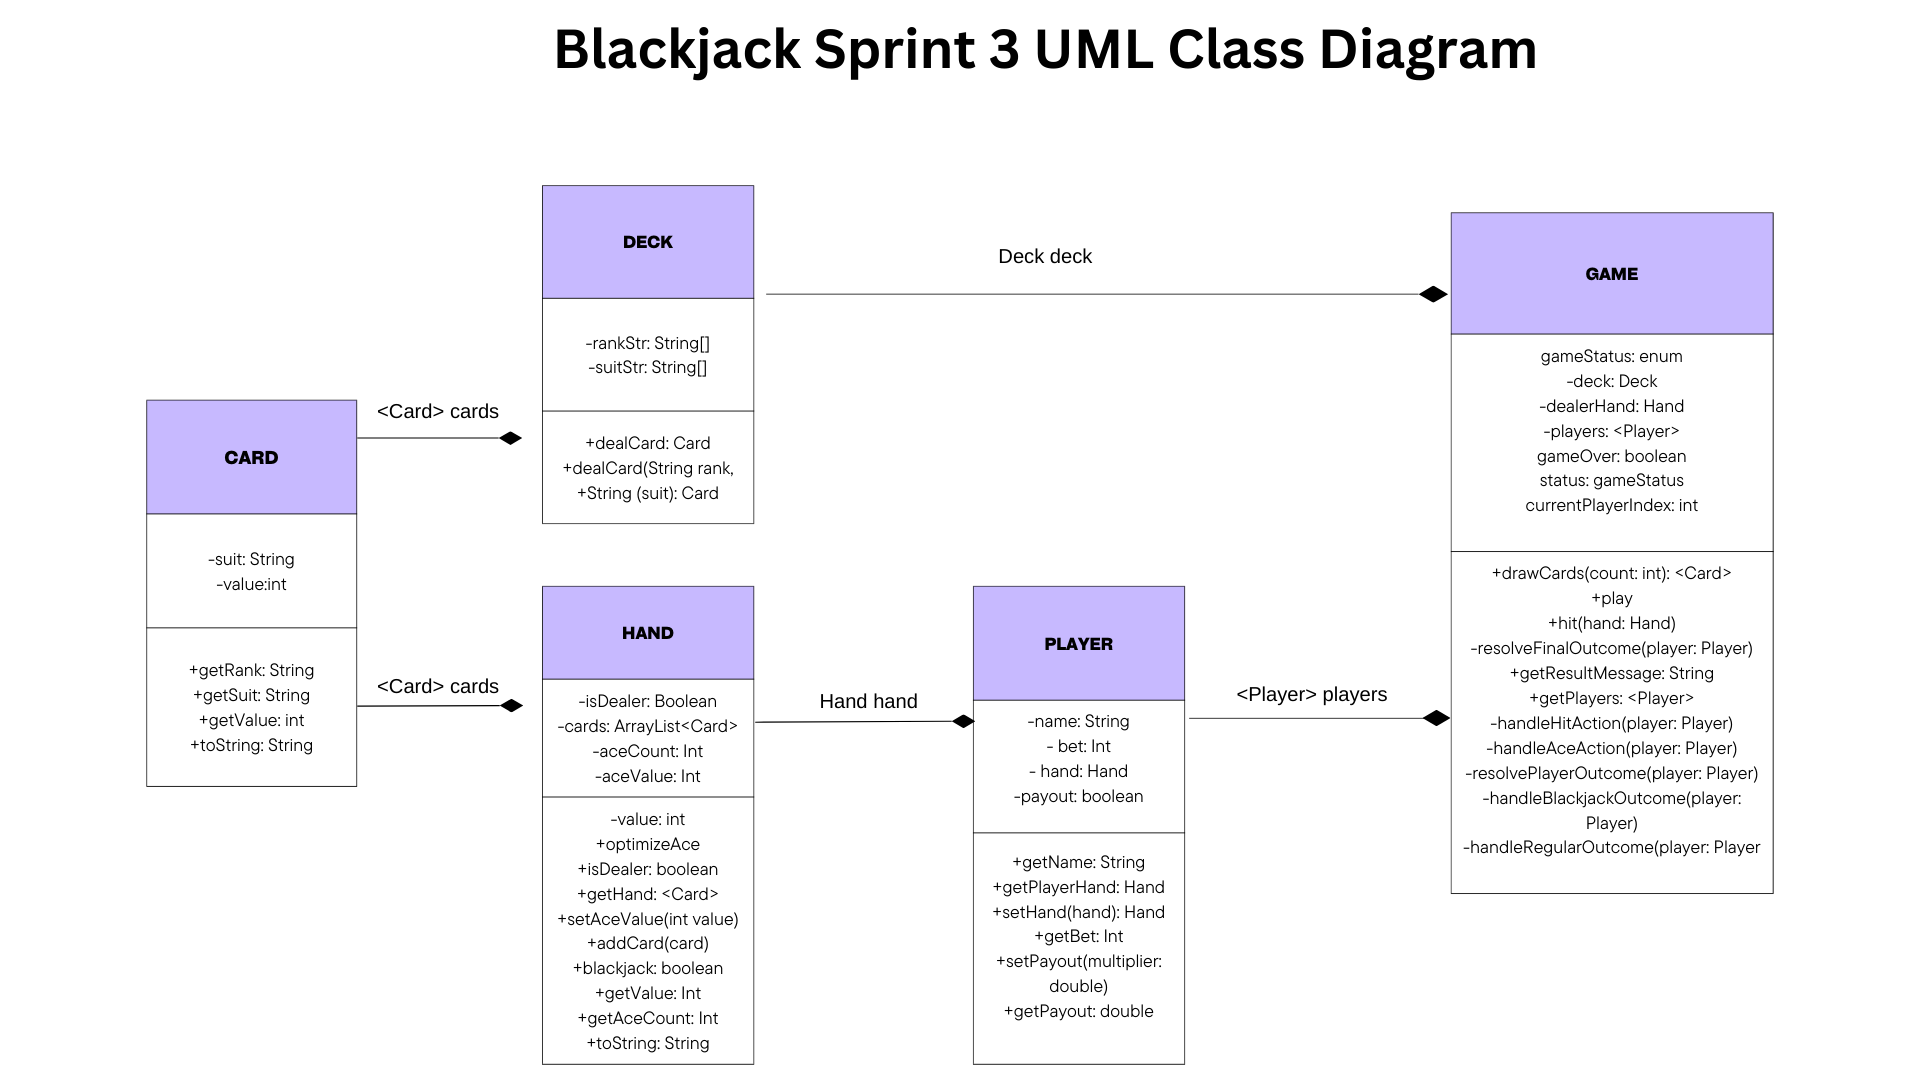
\includegraphics[width=0.5\linewidth]{figures/Sprint_3_UML_Diagram.png}
    \caption{Updated UML diagram for sprint 3}
    \label{fig:sprint 3 UML}
\end{figure}

\noindent This is our updated UML diagram for our model classes and their interactions.


\subsubsection{\colorbox{violet}{(Sprint 3) Retrospective}}
In this sprint we didn't have a lot of things left over from sprint 2. The big ticket item was getting multiplayer functionality done. That task was more challenging and time consuming than anticipated which is why Chris had so many hours for such few points this sprint. The multiplayer aspect was under a 2 point story which in hindsight should've been something along the lines of 5-8 points. Other than that we got a good grove for pace and team dynamic which has been developing over the 3 sprints.


%[[ The requirements analysis identifies \textbf{what} your client wants.
%With each iteration describe the \textbf{how}.
%Include user stories attempted, data structures introduced, and any key design
%decisions.

%Copy this layout for each iteration. ]]


